%!TEX root = ../thesis.tex

\thispagestyle{myheadings}

\graphicspath{{Body/Figures/TrackingFigures/}{Body/Figures/TrackingFigures/MainPlots/}{Body/Figures/TrackingFigures/MainPlots/PlanePlots/}{Body/Figures/TrackingFigures/MainPlots/PullPlots/}{Body/Figures/TrackingFigures/MainPlots/Residuals/}{Body/Figures/TrackingFigures/eLoss/}{Body/Figures/TrackingFigures/CoordSys/}{Body/Figures/TrackingFigures/TrackerPics/}{Body/Figures/TrackingFigures/Field/}{Body/Figures/TrackingFigures/TrackingFlow/}{Body/Figures/TrackingFigures/LeftRight/}{Body/Figures/TrackingFigures/Misc/}{Body/Figures/TrackingFigures/Extrapolation/}{Body/Figures/TrackingFigures/Tracks/}{Body/Figures/TrackingFigures/BeamMeasurements/}{Body/Figures/TrackingFigures/MCDataComparison/}}

\chapter{Track Reconstruction and Analysis}
\label{chapter:TrackReconstruction}

As described in section \ref{sec:StrawTrackers}, the straw trackers are used to provide information about the muon beam, important for the calorimeter \wa analysis, calculating the \wa pitch correction, and determining the spatially weighted magnetic field seen by the muons. The track reconstruction is performed in three stages: First, individual hits in the tracker are grouped into individual tracks in the finding stage. Second, a best trajectory is fit to grouped hits in the fitting stage. Third, the best fit trajectory is extrapolated back to the storage region or forwards to the calorimeter in the extrapolation stage. A fourth refinement stage is planned but not yet implemented, which would add or remove hits in the finding stage based on the results of the fitting and extrapolation stages.

As a brief aside, every stage of the track reconstruction is performed in the event-processing framework known as \textit{art} \cite{art}. The \textit{art} framework is a collection of modularized stages in a C++ framework useful for reading, reconstructing, filtering, analyzing, and writing data, among other things. All Fermilab experiments now use \textit{art}, and E989 is no exception.


\section{Track Finding}
\label{sec:TrackFinding}

The track finding stage consists of pattern recognition routines in order to group individual hits into separate sets corresponding to individual incident tracks. The general implementation of these pattern recognition routines is relatively straightforward \cite{trackfinding,trackfinding2}. Hits across all modules are grouped in time windows called time islands, with a max width of $\SI{100}{ns}$. Within those time islands hits are then grouped into clusters. Clusters consist of one or two hits for each U or V view per module. As a reminder the U and V views of a module consist of the two U or V layers in that module, \secref{sec:StrawTrackers}. Hits are only clustered if they lie in close proximity in time and space to one another. The spatial constraint is defined as the difference in hit straw numbers, from 0 to 31 for the 32 straws per layer, which by default is limited to less than or equal to 4. Neighboring hit clusters in the same module are then grouped to form seeds, one per module. Finally, seeds in successive modules are grouped starting from one end of the tracker to form what are called track candidates. The seeds are formed and grouped into track candidates again only if they lie close in time and space to one another. The entire track candidate formation process occurs for all hits in a time island to find as many real tracks as possible. See \figref{fig:TrackCandidateSelection}.

After a track candidate has been formed a number of checks are made before passing it on to the fitting stage. If hits, clusters, or seeds are found to be shared among multiple track candidates, the candidates are dropped. Likewise, a track candidate is dropped if it is made from seeds consisting of only one type of view, or if the track candidate has less than six hits. There are also various small geometry and timing algorithms to improve the track candidates, such as removing hits from secondaries \cite{trackfinding3}. The $t_{0}$ time for the track candidate is calculated as the mean time of all hits, with some fixed offset at the end. This $t_{0}$ is helpfully constrained by geometry effects, where for a straight track passing through two layers in the same view, the sum of the drift times adds up to a constant (cite or show this?). The track candidate is supplied with an original momentum and position guess at the start of the track by fitting a circle to the hit straw wires in the horizontal plane. The final track candidates are passed on to the fitting stage. 


\begin{figure}[]
    \centering
    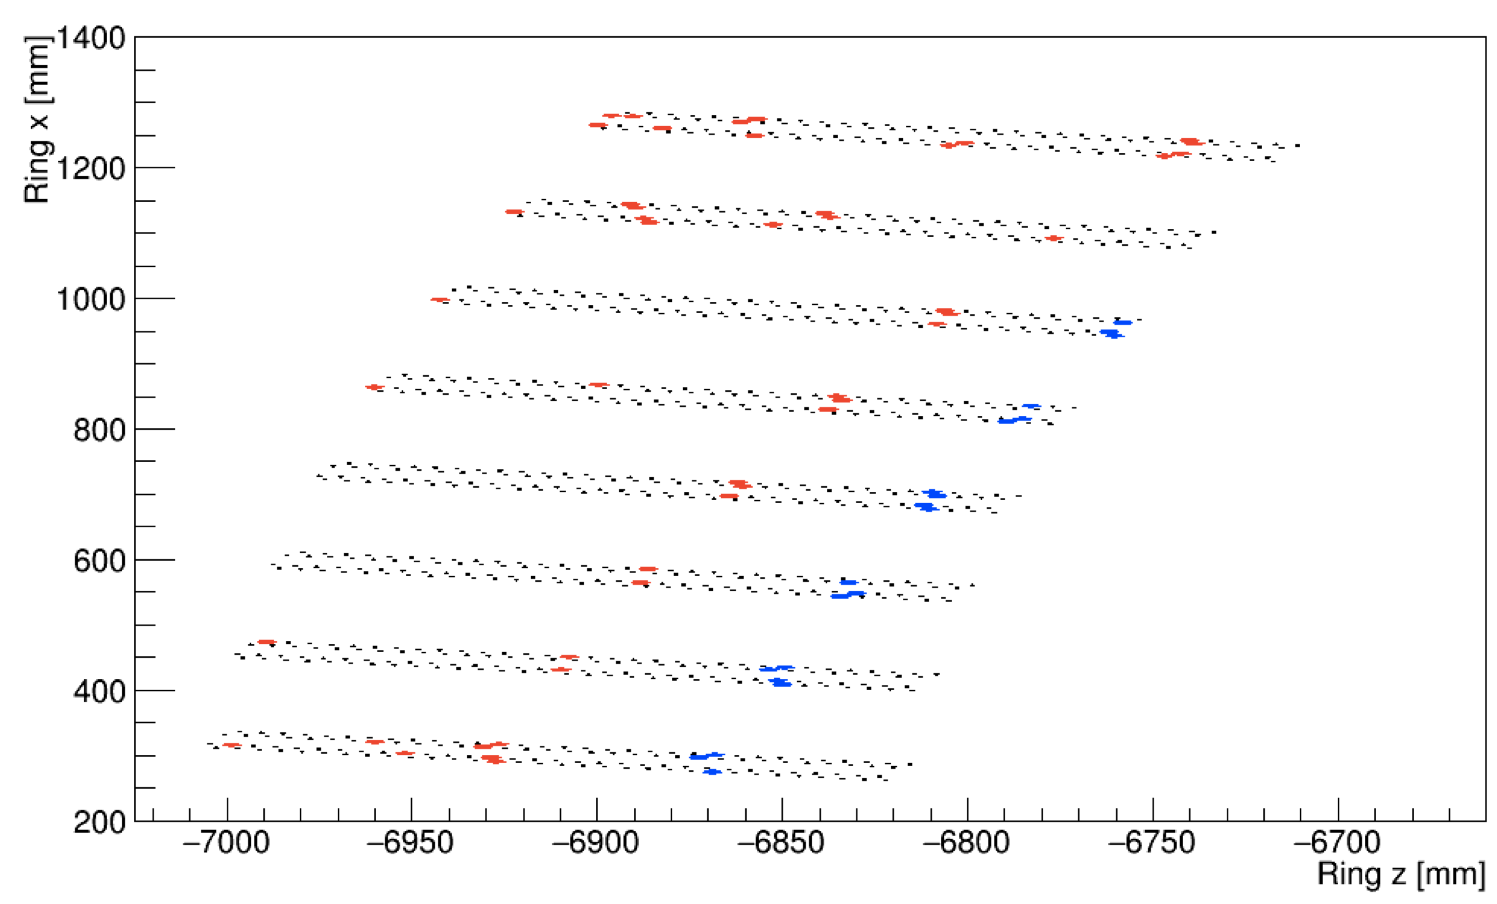
\includegraphics[width=0.9\textwidth]{TrackCandidateSelection}
    \caption[Track candidate selection]{Hits in a tracker station in a single time island. The black dots indicate the position of the straws, while the blue and red points indicate hits. In blue is the first formed track candidate in the island, formed from separate seeds in different modules. The track finding algorithms will move onto the remaining hits in the time island to attempt to form other track candidates, one of which is easily observable by eye.}    
    \label{fig:TrackCandidateSelection}
\end{figure}

% event display tracks

% \begin{figure}[]
% 	\centering
% 	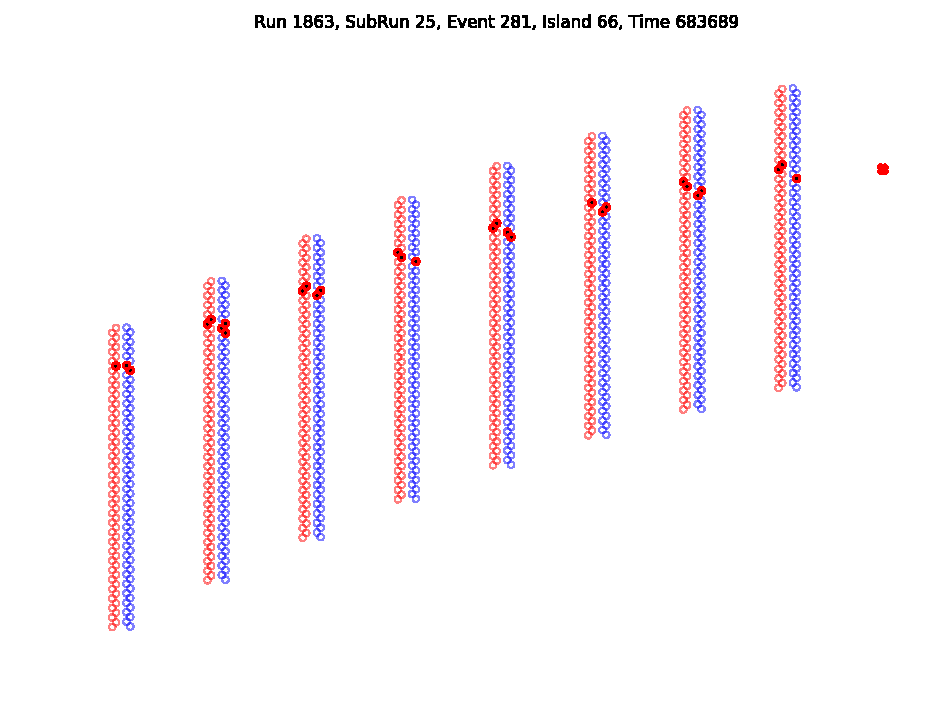
\includegraphics[width=0.9\textwidth]{TrackAndCaloHit}
%     \caption[TrackAndCaloHit]{clean up and possibly replace}    
%     \label{fig:TrackAndCaloHit}
% \end{figure}

% \begin{figure}[]
% 	\centering
% 	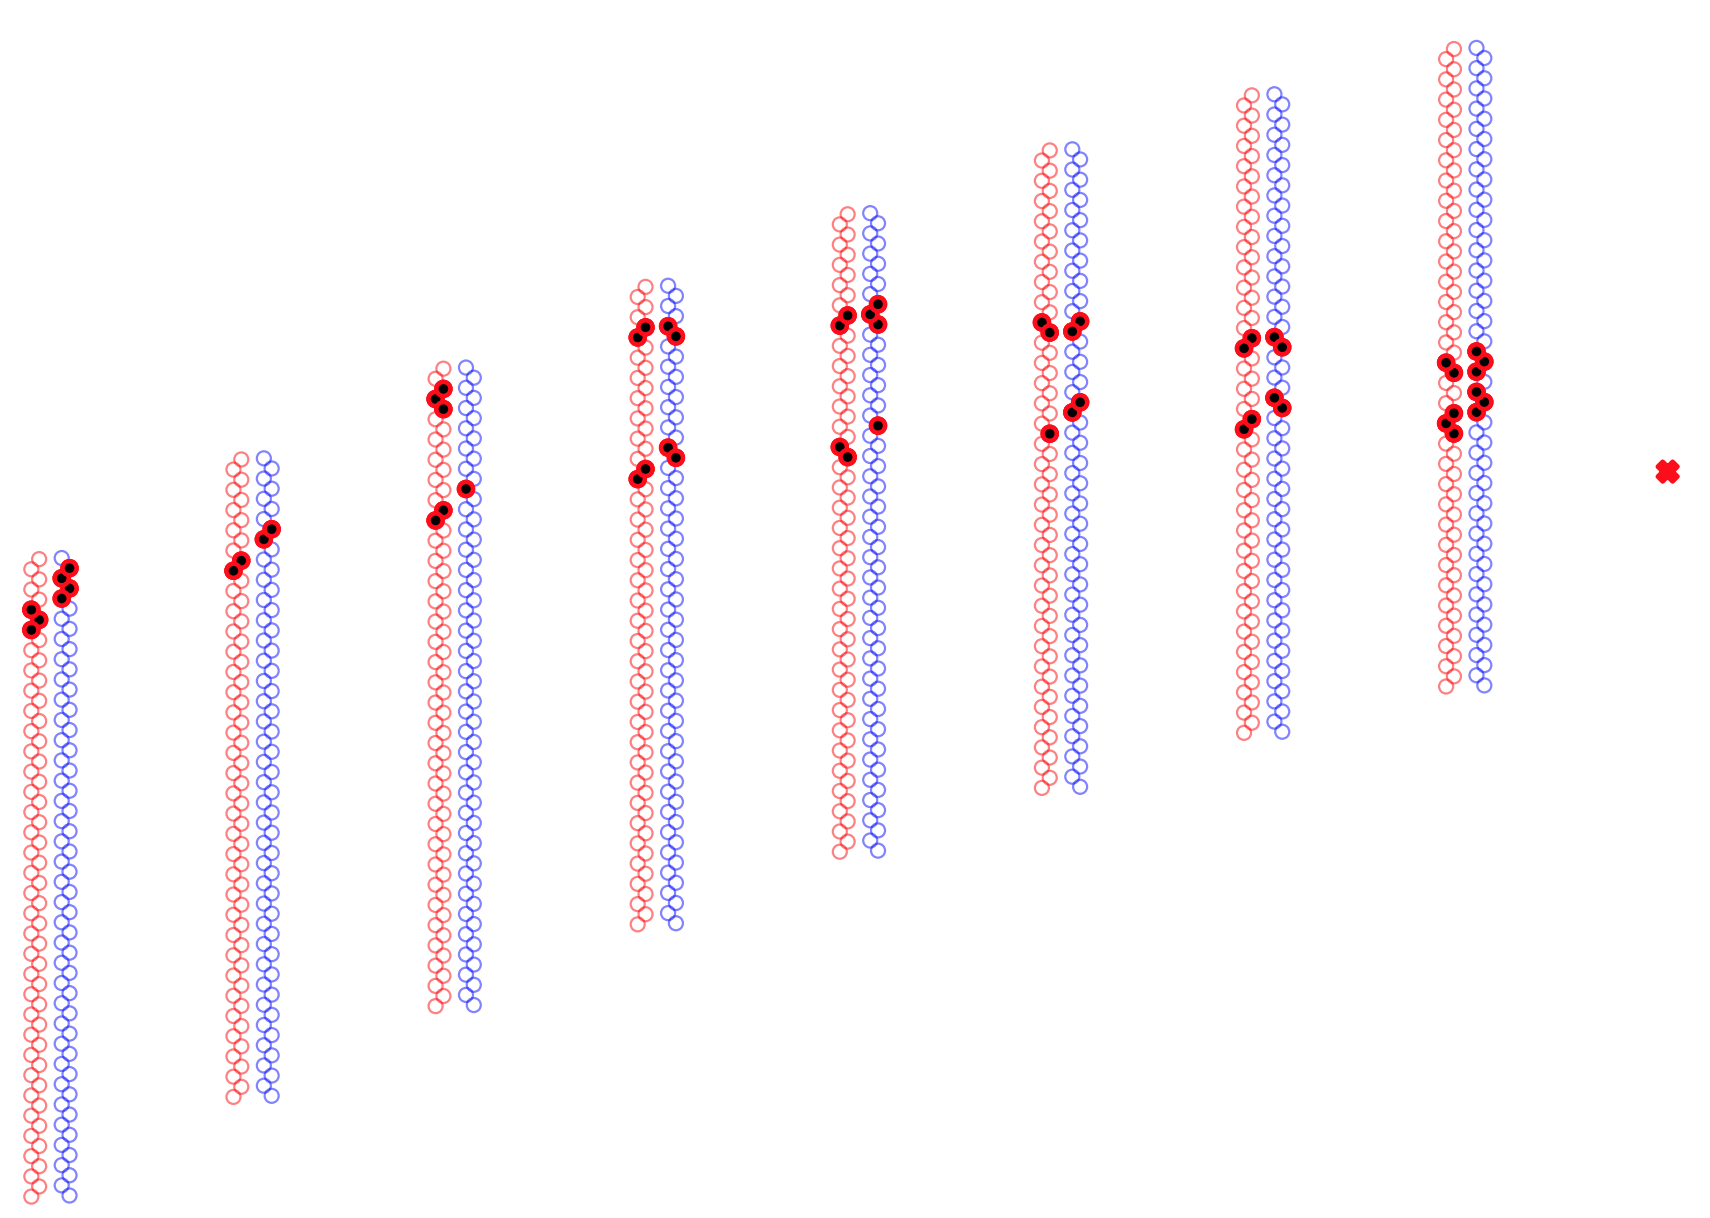
\includegraphics[width=0.9\textwidth]{pileupEvent}
%     \caption[pileupEvent]{clean up and possibly replace}    
%     \label{fig:pileupEvent}
% \end{figure}



\section{Track Fitting}
\label{sec:TrackFitting}


The track fitting stage takes the track candidates from the track finding stage, and outputs a best fit trajectory to those candidates. This includes optimal state vectors and error matrices for the track at each measurement plane and at a ficticious starting plane at the entrance to the straw tracking detector. The track fitting routines can roughly be split into two parts, error propagation and the actual fitting and improvement of the track. The implementation of these parts go hand in hand, and will be described in turn.


\subsection{Error propagation and coordinate systems}

To put it simply, the process of error propagation involves taking track parameters and error matrices (which describe the spread in those track parameters) and transporting them along discrete steps from one point to another, accounting for changes due to any present magnetic fields or material along the step path. There is a set of error propagation routines originally written in Fortran by the EMC collaboration, called ``Geometry and Error Propagation'' or Geane \cite{geanemanual}. Geane works by propagating particles along their average trajectories neglecting the effects of discrete processes, using a helix equation along small enough steps where the change in the magnetic field is small. These routines were used in the E821 experiment as well as the PANDA experiment with some success \cite{Lavezzi}. The Geane routines were at one point converted to C++ and added to Geant4. The strength of using Geane within a Geant4 simulation lies in its direct access to the Geant4 geometry and field. This is crucially important for the E989 track fitting because the trackers live in a region of high field non-uniformity. Shown in \figref{fig:Opera2DFields} is the location of the tracker with respect to the radial and vertical fields. As shown the radial field in the tracker region rises from $\SI{0}{T}$ at the outer ends to roughly $\SI{.3}{T}$ at the inner top and bottom ends, and the vertical field drops approximately 50\% from the storage dipole field of $\SI{1.451}{T}$. These large field gradients over the tracking measurement space must be handled appropriately, which Geane does nicely.



\begin{figure}[]
\centering
    \begin{subfigure}[]{0.75\textwidth}
        \centering
        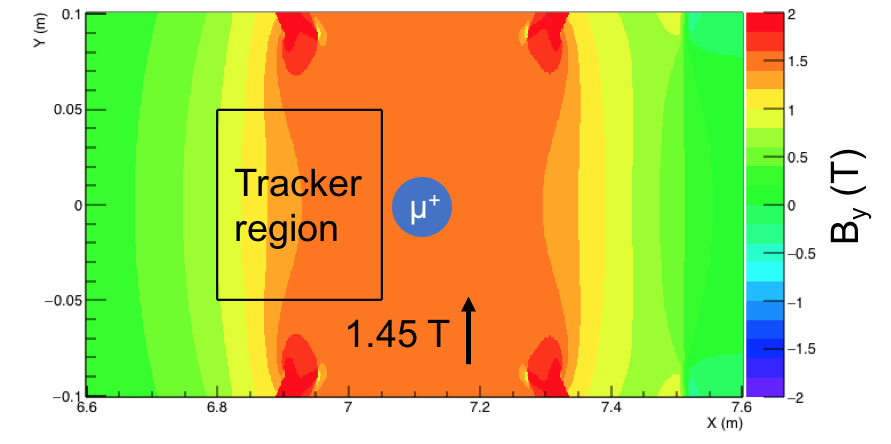
\includegraphics[width=\textwidth]{operaByMod}
        \caption{Vertical magnetic field}
    \label{fig:operaBy}
    \end{subfigure}%
    \vspace{5mm}
    \begin{subfigure}[]{0.75\textwidth}
        \centering
        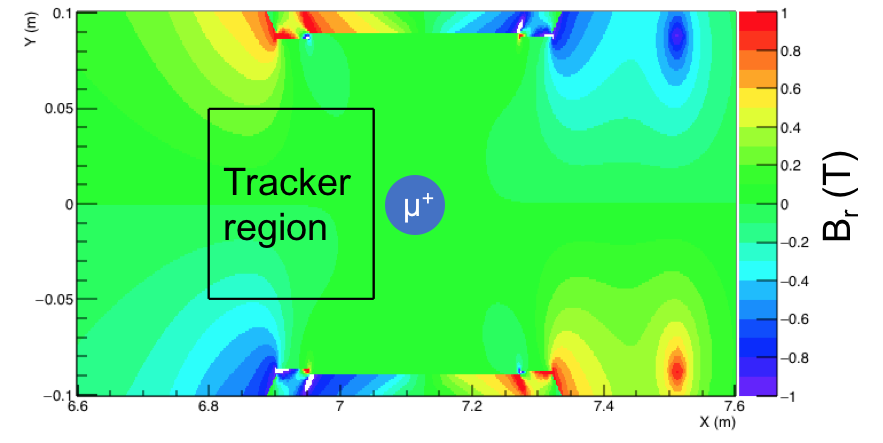
\includegraphics[width=\textwidth]{operaBxMod}
        \caption{Radial magnetic field}
    \label{fig:operaBx}
    \end{subfigure}
\caption[Vertical and radial magnetic fields calculated in Opera2D]{Shown are the vertical (top) and radial (bottom) magnetic fields of the storage ring magnet in and around the storage region as calculated in Opera 2D. The horizontal and vertical axes are the radial and vertical coordinates of the ring respectively. The center of the storage region lies at $\SI{7.112}{m}$ along the horizontal axis. The contours represent the strengths of the vertical and radial magnetic fields. The black box shows the rough location of the tracker with respect to the ring. It can be seen that there is a large field non-uniformity within the tracker space.}
\label{fig:Opera2DFields}
\end{figure}


Predicted track parameters in Geane are a function of path length 
        \begin{align} \label{eq:pp}
            p_{l} = F_{l,l_{0}}(p_{0}),
        \end{align}
where $p_{0}$ are some original tracker parameters and $p_{l}$ are the updated ones. The path length $l$ can be defined or limited how one wishes, and typically corresponds to a single step in the Geant4 simulation. The track parameter vectors $p$ are defined in some coordinate system. In the Geane routines these track parameters are $5 \times 1$ vectors either defined in the ``free'' (curvilinear) system
        \begin{align}
            \frac{1}{p}, \lambda, \phi, y_{\perp}, z_{\perp},
        \end{align}
or the ``surface'' (detector) system 
        \begin{align}
            \frac{1}{p}, \frac{p_{v}}{p_{u}}, \frac{p_{w}}{p_{u}}, v, w.
        \end{align}
In the free system, the $\lambda$ and $\phi$ parameters are the dip $(\pi/2 - \theta)$ and azimuthal angles respectively, while the $y_{\perp}$ and $z_{\perp}$ parameters are defined as being in the $XY$ or $XZ$ global Geant4 planes and orthogonal to $x_{\perp}$, where $x_{\perp}$ is defined as being along the momentum vector of the particle. (Decide whether I want to try and supply a picture showing this here.) In the surface system, the UVW coordinates are defined with any two orthogonal vectors V and W\footnote{For clarification, the UVW surface system has nothing to do with the UV orientations of the straws at this time.}. The surface system is most usefully defined in the tracker reference frame, where the modules are staggered in a local Z coordinate, the local Y coordinate is vertical, and the local X coordinate increases with straw number. See \figref{fig:trackerReferenceFrame}. The surface system is then defined as
        \begin{align}
            \frac{1}{p}, \frac{p_{x}}{p_{z}}, \frac{p_{y}}{p_{z}}, x, y.
        \end{align}
In both free and surface systems the track is represented by one momentum parameter, two directional parameters, and two position parameters. Needing six independent parameters to describe a particle in space and momentum (three momentum and three position parameters), one parameter is left out and taken as a known variable. For Geane this is taken either as a known path length in the free system, or a known U coordinate in the surface system (or known Z coordinate in our tracker reference frame). In our tracker reference frame, the 32 straw layers corresponding to a tracking station are defined at known local Z coordinates. The path lengths for steps in Geane can be set to be equal to the distance for a track to travel between between detector planes, and therefore the track parameter dependence on the path length can instead by replaced by a dependence on plane number.


\begin{figure}[]
  \centering
  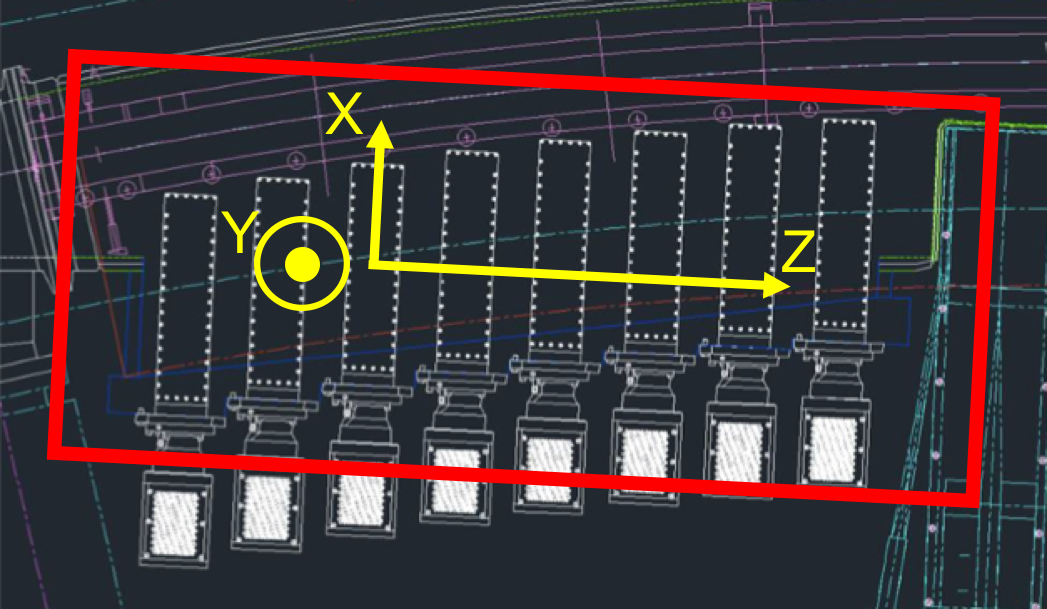
\includegraphics[width=0.7\textwidth]{trackerReferenceFrame}
    \caption[Tracker reference frame]{Shown is a model view of a tracker station in relation to the magnetic ring. Tracker modules are shown in white. Around the tracker measurement area is defined a coordinate system called the tracker reference frame. In that frame, the X coordinate is directed outward along the straws nearly radially, the Y coordinate is directed vertically up, and the Z coordinate is directed along the direction that the tracker modules are staggered.}
    \label{fig:trackerReferenceFrame}
\end{figure}


The $5 \times 5$ error matrix on a plane calculated in Geane describing the expected distribution in true parameters about the average ones is defined as
    \begin{align} \label{eq:sigma}
        \sigma_{N}^{ij} = <p_{N}^{i}p_{N}^{j}> - <p_{N}^{i}> \cdot <p_{N}^{j}>,
    \end{align} 
where i and j are track parameter indices and $N$ is some plane number. This error matrix will include effects from multiple scattering, delta ray production, ionization, and bremsstrahlung \cite{geanemanual,energyloss}. These matrices are transported from plane to plane by what are called transport matrices, where the $5 \times 5$ transport matrix elements between two planes are defined as 
    \begin{align}
        T_{N,N-1}^{i,j} = \frac{\partial p^{i}_{N}}{\partial p^{j}_{N-1}}.
    \end{align}
The transport matrix $T$ is a Jacobian between planes which expresses the infinitesimal changes in parameters at some plane (or path length) with respect to the parameters at some previous plane (or previous path length):
    \begin{align} \label{eq:transport}
        \delta p_{N} &= T_{N,N-1} \delta p_{N-1}
    \end{align}
The error matrix is propagated forward from one plane to another by
    \begin{align} \label{eq:transport}
        \sigma_{N} &= T_{N,N-1} \sigma_{N-1} T_{N,N-1}^{T} + \sigma_{\text{material}},
    \end{align}
where $\sigma_{\text{material}}$ is the added error due to material effects between the planes. The calculation of the transport matrices themselves is done within the Geane routines in the free system on a step by step basis, where the derivation of the transport matrix elements is given in \refref{jacob}. It should briefly be pointed out that the transport matrix between any two planes (or number of steps) is the multiple of all intermediate transport matrices,
    \begin{align}
        T_{N,N-2} = T_{N,N-1} T_{N-1,N-2},
    \end{align}
regardless of what reference system the matrices are defined in (as long as they are all consistent). Geane can convert the transport matrices between the free system and the surface system using further Jacobians, also derived in \refref{jacob}. When converting a transport matrix from one reference system to another,
    \begin{align} \label{eq:Ttransform}
        T_{N,N-1}^{s} = A_{N} T_{N,N-1}^{f} A_{N-1}^{-1},
    \end{align}
where the $s$ and $f$ superscripts stand for the surface and free reference systems respectively, and $A$ is the Jacobian between reference frames which is defined at a specific point or plane $(A_{N} \neq A_{N-1})$. The error matrices are converted between reference frames in the usual way, 
    \begin{align} \label{eq:Sigtransform}
        \sigma_{N}^{s} &= A_{N} \sigma_{N}^{f} A_{N}^{T}.
    \end{align}


Finally, while the tracker reference frame is nominally defined in the local XYZ coordinates as described previously, the straws themselves don't measure in that frame directly. As described in \secref{sec:StrawTrackers}, the straws measure drift circles in planes perpendicular to the straws themselves. The measurements from U and V straws therefore lie on the U and V measurement axes shown in \figref{fig:GeaneCoordSys}, where the measurement of the drift circle is instead taken as a U or V coordinate to the left or right of the straw wire. The new coordinate system is therefore defined as
        \begin{align}
            \frac{1}{p}, \frac{p_{u}}{p_{z}}, \frac{p_{v}}{p_{z}}, u, v,
        \end{align}
where this $Z$ variable is the tracker reference frame $Z$, and the transformation between the $XYZ$ and $UVZ$ systems is given by
    \begin{align}
        p^{UV} &= J_{5} p^{XY} \\
    \end{align}
where $J_{5}$ is a $5 \times 5$ matrix defined by
        \begin{align}
            J_{5} = 
            \begin{pmatrix}
                1 & 0 & 0 \\
                0 & J_{2} & 0 \\
                0 & 0 & J_{2}
            \end{pmatrix}
        \end{align}
and $J_{2}$ is a $2 \times 2$ matrix given by
        \begin{align}
            \begin{pmatrix}
                u \\
                v \\
            \end{pmatrix} =
            J_{2}
            \begin{pmatrix}
                x \\
                y \\
            \end{pmatrix} =
            \begin{pmatrix}
                \cos{\theta} & -\sin{\theta} \\
                \cos{\theta} & \sin{\theta} \\
            \end{pmatrix}
            \begin{pmatrix}
                x \\
                y \\
            \end{pmatrix}.
        \end{align}
In order to transform the transport or error matrices from the tracker reference frame to the tracker measurement frame, the same relations as in Equations~\ref{eq:Ttransform} and \ref{eq:Sigtransform} apply,
    \begin{align}
        T_{N,N-1}^{UV} &= J_{5} T_{N,N-1}^{XY} J_{5}^{-1} \\
        \sigma_{N}^{UV} &= J_{5} \sigma_{N}^{XY} J_{5}^{T}
    \end{align}
where the superscripts of $XY$ or $UV$ identify which coordinate system the objects belong to. It's important to note that out of the five track parameters each straw only measures only a single U or V position. 

\begin{figure}[]
  \centering
  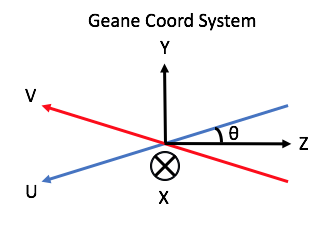
\includegraphics[width=0.5\textwidth]{GeaneCoordSys}
    \caption[Natural tracker measurement system]{The straw tracker measurement reference system. The XYZ system here is the straw tracker reference frame. $\theta$ is the same angle as the stereo angle of the straws, at 7.5\textdegree{}. U straws measure along the U axis and V straws measure along the V axis.}
    \label{fig:GeaneCoordSys}
\end{figure}





% \appref{app:transportmatrixproperties}





\clearpage



-cite james thing









the transformation between the two is handled in the code and given by reference .. 


Geane does everything in the free system and converts to the surface system ... 

transport matrices are calculated in ...


step by step vs plane by plane

inverse vs transpose


-it was found that doing the minimization in UV space removed correlations (cite James here) instead of XY, docdb 3813

-make sure to cite traj fit paper


-fit in GeV cm vs MeV mm



-need to see what I've written down below, and what I might move up here and such

-average path
-helix
-cite proper stuff

-need to talk about material effect calculations
-reference frames and multiplication of matrices to go between them
-transport and error matrix calculations
-eq 4.5 not quite right


measurement error being the largest error ... 


-don't forget to cite my track fitting note probably



\subsection{\texorpdfstring{\chisq}{chisq} minimization}
% \label{sec:TrackFittingFormalism}


-globabl chi2 minimization
-other fitting algortihms could be used, kalman filter by lavezzi



    I recommend reading \cite{geanemanual}, Chapter 4 of \cite{Lavezzi}, and \cite{trajfit} in order to best understand the fitting algorithm. However, due to the at times confusing notation, ommitted equations or concepts, and differences between papers, I have attempted to summarize here the different sources and present the material in a more understandable and readable format. The implementation of the fitting algorithm into the code follows this section.

    One can define a $\chi^{2}$ for a track in the usual way by dividing the residuals of measured and predicted track parameters by their errors:
        \begin{align} \label{eq:chi2}
            \chi^2 = (\vec{p}-\vec{x})^{T} (\sigma^{-1}) (\vec{p}-\vec{x}),
        \end{align}
    where $\vec{p}$ are predicted track parameters from a fit to the measured track parameters $\vec{x}$, and $\sigma$ is a covariance matrix of errors on the fitted parameters. The Geant4 error propagation routines can be used to determine these predicted parameters and error matrices by propagating track parameters from some initial guesses. By minimizing this $\chi^{2}$ with respect to the track parameters one can then fit and improve the track. 



    % The Geant4 error propagation routines propagate particles along their average trajectories neglecting the effects of discrete processes, using a helix equation along small enough steps where the change in the magnetic field is small. The predicted parameters are then a function of path length: 
    %     \begin{align} \label{eq:pp}
    %         p_{l} = F_{l,l_{0}}(p_{0}),
    %     \end{align}
    % where the path length can be defined how one wishes. 




    % In tandem, error matrices describing the expected distribution in true parameters about those predicted parameters due to said discrete process are also calculated:
    %     \begin{align} \label{eq:sigma}
    %         \sigma^{ij} = <p^{i}p^{j}> - <p^{i}> \cdot <p^{j}>,
    %     \end{align} 
    % where i and j are track parameter indices. These parameter vectors are 5x1 objects defined in some track representation, as described in the \hyperref[sec:Coord]{Coordinate Systems} section. The propagation of these parameters and error matrices are done using transport matrices, which express the infinitesimal changes in parameters at some plane (or path length) with respect to the parameters at some previous plane (or previous path length):
    %     \begin{align} \label{eq:transport}
    %         \delta p_{N} &= T_{N,N-1} \delta p_{N-1}, \\
    %         \sigma_{N} &= T_{N,N-1} \sigma_{N-1} T_{N,N-1}^{T}.
    %     \end{align}
    % Said transport and error matrices are 5x5 objects since the parameter vectors are 5x1 objects as described above. The calculation of these transport matrices, as well as details on the functional form of \ref{eq:pp} are shown in \cite{jacob}.

    With parameters defined on such planes, one can define the $\chi^{2}$ as: 
        \begin{align} \label{eq:chi2sum}
            \chi^2 = \sum_{i=1}^{N} [(p_{i}(p)-x_{i})^{T} (\sigma_{i}^{-1}) (p_{i}(p)-x_{i})],
        \end{align}
    where $p_{i}$ are the average predicted parameters from some general starting parameters $p$. At first order one can solely include the measurement errors on parameters, which fill in the diagonals of $\sigma_{i}$, if random processes can be neglected. Unmeasured parameters should have measurement errors of infinity (or some large value) along the diagonals in the code, which account for the fact that residuals for unmeasured parameters do not exist. When the error matrix is inverted all rows and columns of the matrix with these large numbers will fall to 0 in the $\chi^{2}$. 

    In order to get the best fit track, the $\chi^{2}$ should be minimized with respect to the initial track parameters p, and evaluated at some chosen or fitted parameters:
        \begin{align} \label{eq:minimize}
            \frac{\partial \chi^{2}}{\partial p}|_{p=p'_{0}} = 0,
        \end{align}
    resulting in
        \begin{equation}
        \begin{aligned}
            0 = \sum_{i=1}^{N}[ (\frac{\partial p_{i}(p)}{\partial p}|_{p=p'_{0}})^{T} (\sigma_{i}^{-1}) (p_{i}(p'_{0})-x_{i}) \\ 
            + (p_{i}(p'_{0})-x_{i})^{T} \frac{\partial(\sigma_{i}^{-1})}{\partial p}|_{p=p'_{0}} (p_{i}(p'_{0})-x_{i}) \\ 
            +  (p_{i}(p'_{0})-x_{i})^{T} (\sigma_{i}^{-1}) (\frac{\partial p_{i}(p)}{\partial p}|_{p=p'_{0}})]
        \end{aligned}
        \end{equation}
    where the 1st and 3rd terms are identical, and the 2nd term is small if one assumes that the error matrix doesn't change much with respect to the starting parameters. (Fair since most of the error comes from measurement, and as long as the initial guess is decent enough such that the path length through material doesn't change appreciably from one iteration to the next.) This simplifies to: 
        \begin{align} \label{eq:solve}
            \sum_{i=1}^{N} T^{T}_{i0} (\sigma_{i}^{-1}) (p_{i}(p'_{0})-x_{i}) = 0,
        \end{align}
    which is just the top term with 
        \begin{align} \label{eq:transport2}
             T_{i0} = \frac{\partial p_{i}(p)}{\partial p}.
        \end{align}
    To solve this make the substitution 
        \begin{align} \label{eq:psub}
            p_{i}(p'_{0}) = p_{i}(p_{0}) + \frac{\partial p_{i}(p_{0})}{\partial p} \Delta p_{0} = p_{i}(p_{0}) + T_{i0} \Delta p_{0},
        \end{align}
    where $p'_{0}$ are the improved starting parameters for the next iteration calculated from the previous starting parameters $p_{0}$, and $\Delta p_{0}$ are the changes in the starting parameters to improve the track. This equation can be plugged into the above if one makes the assumption that $T_{i0}$ does not change much from one iteration the next, which follows from the inherent nature of making small adjustments to the track in order to improve it.

    After simplifying one arrives at 
        \begin{align} \label{eq:deltap}
            \Delta p_{0} = \sigma_{p_{0}} \sum_{i=1}^{N} T^{T}_{i0}(\sigma_{i}^{-1})(x_{i} - p_{i}(p_{0})),
        \end{align}
    where
        \begin{align} \label{eq:cov}
            \sigma_{p_{0}} = [\sum_{i=1}^{N} T^{T}_{i0} (\sigma_{i}^{-1}) T_{i0} ]^{-1},
        \end{align}
    is the 5x5 covariance matrix of fitted parameters on the starting plane, whose diagonals describe the errors in the 5 track parameters on that plane and in the region close to it. (The fit does not directly return fit errors for track parameters on other planes.) $\Delta p_{0}$ along with $\chi^2$ is exactly what we want to determine since that is what allows us to fit and improve the track from iteration to iteration.

    However, since random processes should not be neglected for optimal tracking results, it makes more sense to return to the original $\chi^2$ in equation \ref{eq:chi2}, only now the included matrix and vector objects are combined into one large linear algebra equation. Instead of a sum over N 5x1 objects multiplying 5x5 error matrices, the vectors are combined into a single 5Nx1 vector multiplying a single 5Nx5N matrix. The 5x5 diagonal blocks of this large error matrix should now include the effects due to material processes as calculated in Geant from equation \ref{eq:sigma} as well as the measurement errors. 

    Because now parameters at one plane are no longer independent of the parameters at other planes, due to correlations from these random processes, it's necessary to add off-diagonal elements into the large error matrix. These 5x5 blocks come from 
        \begin{align} \label{eq:corr}
            \sigma_{MN} = T_{MN} \sigma_{N}, 
        \end{align}
    for the top diagonals, and the transpose for the bottom diagonals, where M and N are two separate planes within the detector. ($\sigma_{N}$ is the error matrix on plane N calculated from the starting plane.) This follows from equation \ref{eq:sigma} evaluated at plane M with respect to a path length from plane N, and not plane 0, which is equivalent to \ref{eq:corr}. 

    You can then minimize the $\chi^{2}$ in the same way, only again with the matrix objects being aggregates of the per plane objects:
        \begin{align} \label{eq:deltafull}
            \Delta \vec{p}_{0} = \sigma_{p_{0}} \tau^{T}\sigma^{-1}(\vec{x}-\vec{p}),
        \end{align}
        %
        \begin{align} \label{eq:covfull}
            \sigma_{p_{0}} = [\tau^{T} \sigma^{-1} \tau ]^{-1},
        \end{align}
    where $\tau$ is the combined transport matrices from the individual 5x5 matrices, a 5Nx5 object.

    The unmeasured parameter errors of infinity still come into play in the final calculation in the same was as before. Because however these matrix objects are very large, and the tracking must have a certain amount of speed in order to keep up with data, it is useful to reduce the size of these matrices. (It also makes things easier programming wise. Note that there are other some other ways to speed things up, specifically the banded inversion method as described in reference \cite{trajfit}. This method was not used in favor of getting the code working in the simpler form in the first place, but it is a possibility in the future to use this technique to speed things up even more.) It suffices to simply remove all rows and columns where said infinity values exist in the error matrix. This is mathematically equivalent to inverting the error matrix with the infinities included, which make all rows and columns where they exist go to zero. The associated unmeasured parameter rows in the residual vector and transport matrices must similarly be removed. This results in an Nx1 residual vector, NxN error matrix, 5xN combined transport matrix transpose, which multiply against the 5x5 covariance matrix out front to still result in a 5x1 fix to the starting parameters, and a scalar $\chi^2$ value. (Note that these element removals should be done just before the final calculation, and not higher up in the algebra, otherwise plane correlations are not properly calculated.)

    By calculating the last two equations one can fit the track, acquire a $\chi^{2}$ describing the degree of the fit, determine how the track parameters can be improved at the starting point, and calculate errors on those starting parameters. This algorithm can be iterated a number of times to get a best fit track until successive iterations produce no improvement, where usually 3 or 4 iterations is enough. Note that there is remarkable robustness with respect to the initial starting parameters in fitting the track. Of course if the initial starting parameters are too poor, then the fit will not converge. All of these calculations are completed within the \hyperref[sec:GeaneFitter]{GeaneFitter.cc} file within the framework.







% Structure for the track fitting section:
% 1. Introduction to Geane and what it gives you, why we use it, etc.
% 2. Explanation of chi2 fitting routine used, brief mention of other possible fitting possibilties
%     1. Material correlations
%     2. Which parameters are measured and which aren't
%     3. Jacobians and transformations used everywhere
%         1. Probably some math on this last guy
% 3. Types of fitting used, various modes and options
%     1. Left-right ambiguity
% 4. Plots and images everywhere showing what all I've done



\subsection{Left right ambiguity}
\label{sub:leftright}



\subsection{Plots and results and stuff}


-go into all tests and pieces of the code
-vacuum fitting
-chi2 plot and overlayed red curve for x ndf
-checks on energy loss
-material correlation code
-fast fitting code
-different fitting modes
-mc / data comparisons
-don't forget about angular correction in appendix of fitting documentation - might want to put that in the appendix of my thesis
-red black point residual plots too maybe
-talk about the dummy stuff too perhaps
-ficticious starting plane


-should talk about geometry determination of hits in straws which I havent yet - in the fitting side of things though - see Joes docdb 6947 to start (maybe others too) - for LR determination after wire fit (but only in full sequence fit I believe...)




\begin{figure}[]
  \centering
  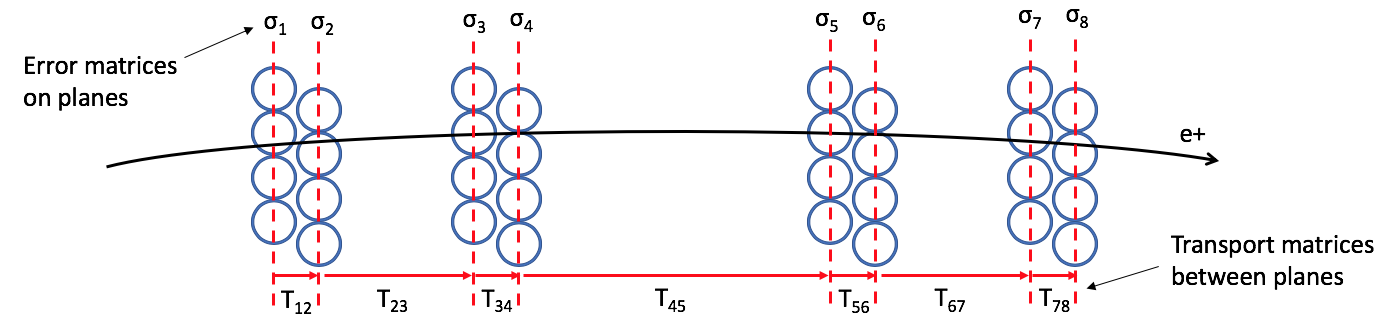
\includegraphics[width=\textwidth]{FittingMatricesDiagram}
    \caption[Fitting matrices diagram]{}
    \label{fig:FittingMatricesDiagram}
\end{figure}

\begin{figure}[]
  \centering
  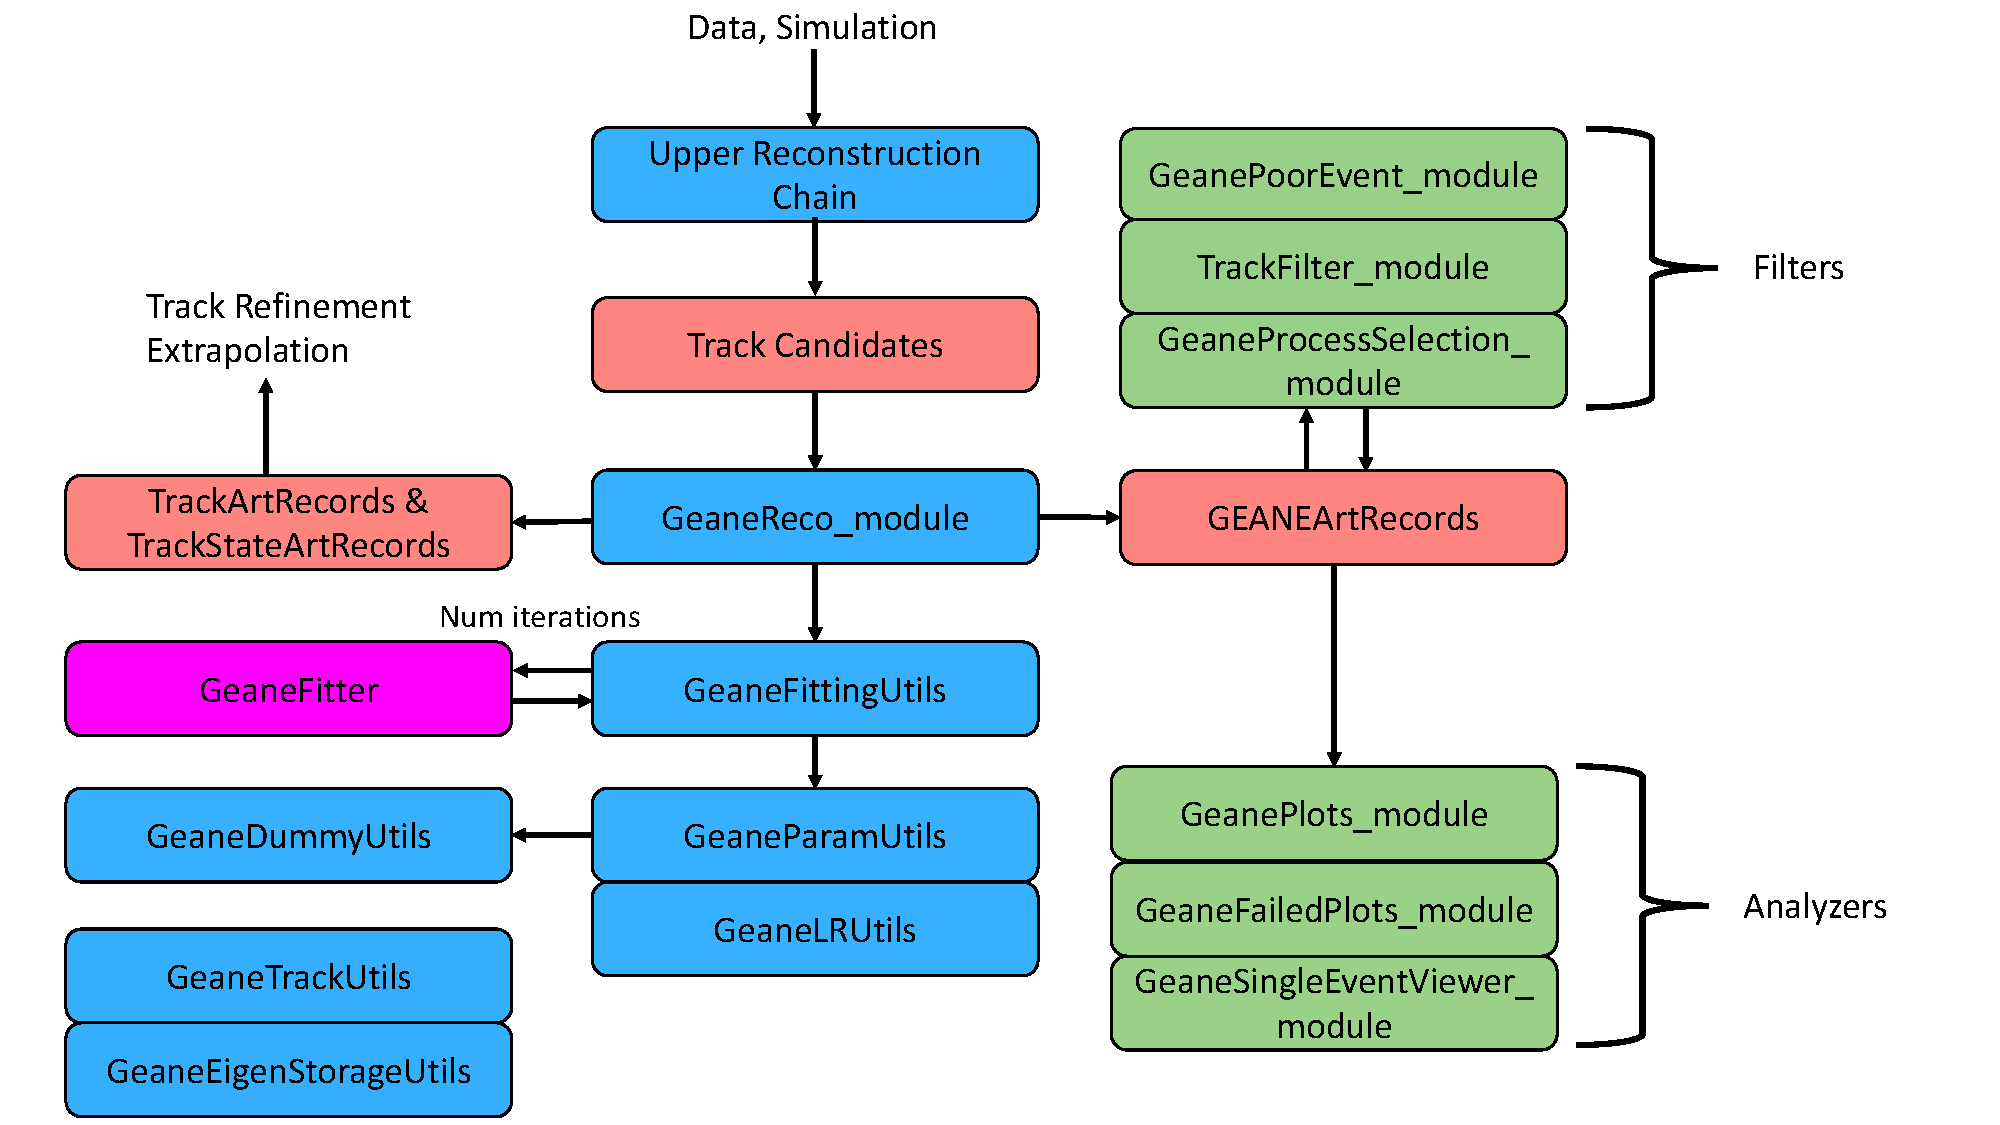
\includegraphics[width=\textwidth]{NewGeaneFlow}
    \caption[Geane code flow]{}
    \label{fig:NewGeaneFlow}
\end{figure}



\section{Track Extrapolation}
\label{sec:TrackExtrapolation}

The last stage of the track reconstruction is the track extrapolation. The extrapolation takes the fitted track results and either extrapolates them back to the storage region to the approximate position of the muon decay point, or forwards to the face of the calorimeter sitting right behind the tracker. The extrapolation stage utilizes a fourth order Runge-Kutta Nystr\"{o}m algorithm \cite{SCThesis} which discretely steps a trajectory through the magnetic field in the full \gmtwo Geant4 simulation, similar in some respects to the track fitting stage. At each step of the extrapolation, the updated track position and covariance matrix are compared to physical volumes in the simulation to flag tracks which have been reconstructed as likely originating from outside the storage region \cite{SCThesis,extrapolationerrors}. Because there is no fixed interaction point in the storage region, tracks are extrapolated backwards to the point of tangency where the radial momentum is equal to zero. Studies were done to verify that this approximation for the muon decay point was sufficient using truth Monte-Carlo, and it was found that a simple $\SI{1.1}{mm}$ correction to the radial decay position could be applied regardless of the momentum of the track \cite{SCThesis}. The vertical extrapolated distribution was found to have no biases. (What about the azimuthal point? Mentioned a little bit in DocDB 8564 but do I really want to go into it?) A birds eye view for extrapolation results is shown in \figref{fig:VertexPlanView}. A radial slice of the extrapolated beam distribution is shown in \figref{fig:BeamCrossSection}.


\begin{figure}[]
    \centering
    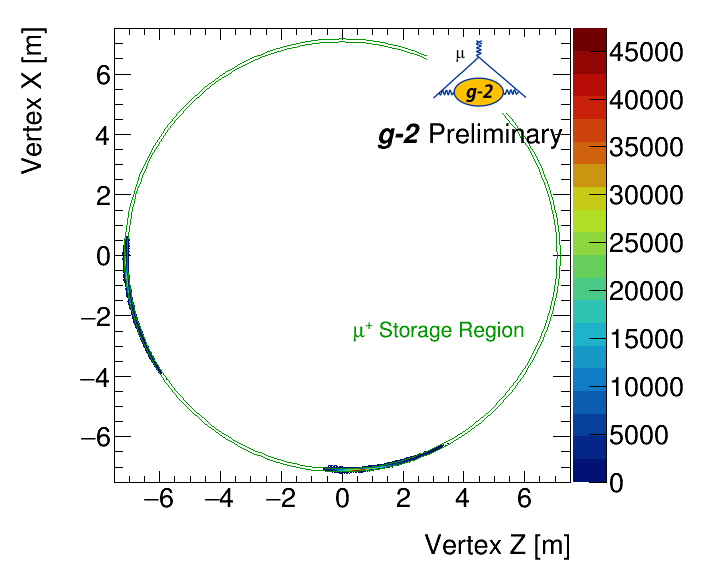
\includegraphics[width=\textwidth]{VertexPlanView}
    \caption[Birds eye view of extrapolation in ring]{A birds eye view of the extrapolation results in the storage ring. The two distributions of extrapolated tracks can be seen at the left and bottom of the figure, where the tracker sits at the heads of the distributions. It can be seen that some tracks are extrapolated multiple meters back through the storage region. (Mention anything about the cuts in this plot?)}    
    \label{fig:VertexPlanView}
\end{figure}

\begin{figure}[]
  \centering
  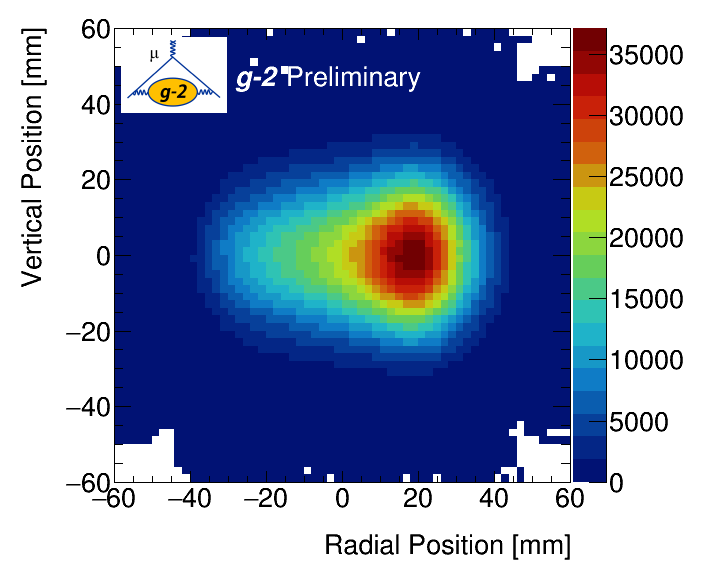
\includegraphics[width=0.7\textwidth]{BeamCrossSection}
    \caption[Extrapolated muon beam distribution cross-section]{Shown is a radial slice of the extrapolated muon distribution or beam spot. The beam is localized off center of the storage ring due to the kicker settings used, \secref{sub:kicker}. (Mention that last bit at all? Mention anything about the cuts in this plot?)}
    \label{fig:BeamCrossSection}
\end{figure}








\section{Muon Beam Measurements}
\label{sec:MuonBeamMeasurements}

-for showing plots include a bulleted list or table of the tracking cuts made

-emphasize measurements that are directly relevant to the calorimeter \wa analysis
-cbo frequency
-cbo amplitude
-have a CBO subsection alongside general results? 





\begin{figure}[]
    \centering
    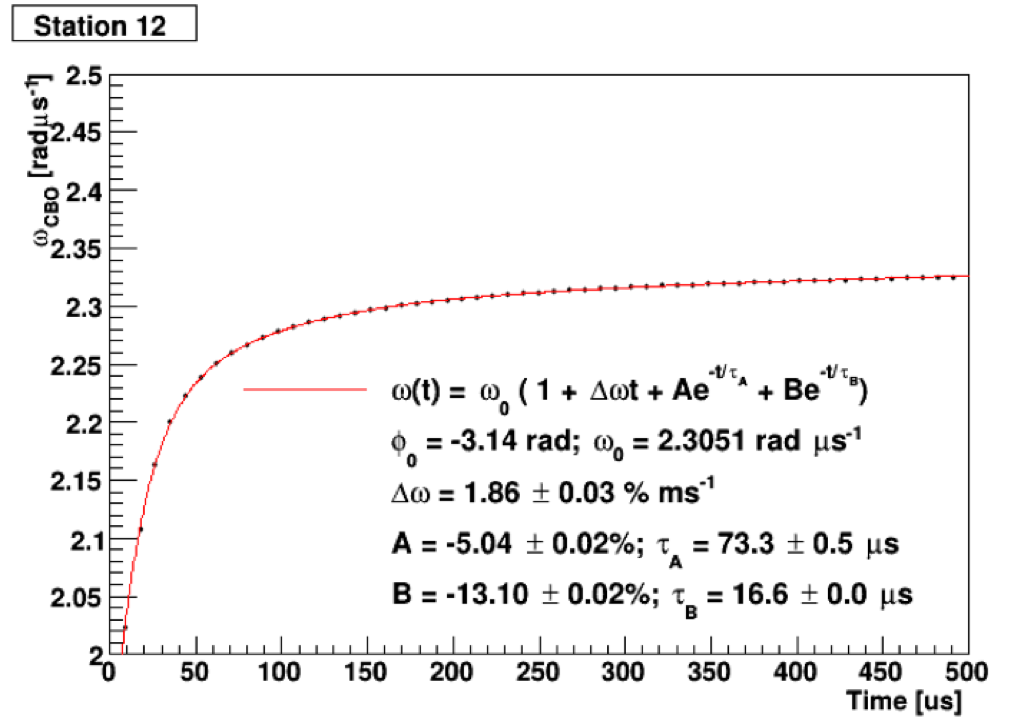
\includegraphics[width=0.9\textwidth]{CBOFrequency}
    \caption[CBO frequency]{}    
    \label{fig:CBOFrequency}
\end{figure}

\begin{figure}[]
    \centering
    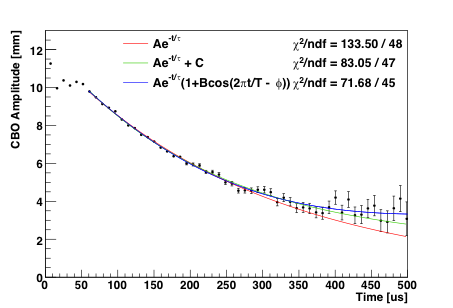
\includegraphics[width=0.9\textwidth]{CBOAmplitude}
    \caption[CBO amplitude]{}    
    \label{fig:CBOAmplitude}
\end{figure}



\clearpage


-in all pictures of this chapter (and others too), make sure to to go back through figures and check that I've given credit properly



